\documentclass[11pt]{article}
\usepackage[a4paper,margin=25mm]{geometry}
\usepackage{amsmath,amssymb,amsthm,mathtools,booktabs,graphicx,microtype,xcolor}
\usepackage[T1]{fontenc}
\usepackage{lmodern}
\usepackage[colorlinks=true,linkcolor=teal,citecolor=teal,urlcolor=teal]{hyperref}
\usepackage{enumitem,fancyhdr,listings}
\setlist{nosep,leftmargin=*}
\newtheorem{theorem}{Theorem}
\newtheorem{proposition}[theorem]{Proposition}
\newtheorem{corollary}[theorem]{Corollary}
\theoremstyle{definition}\newtheorem{definition}[theorem]{Definition}
\newcommand{\Z}{\mathbb Z}
\newcommand{\F}{\mathcal F}
\newcommand{\B}{\mathcal B}
\newcommand{\C}{\mathcal C}
\DeclareMathOperator{\lcm}{lcm}
\pagestyle{fancy}\fancyhf{}\fancyhead[L]{\small Source-aware modular reconstruction}\fancyhead[R]{\small Shivam Gupta}\fancyfoot[C]{\thepage}
\setlength{\headheight}{14pt}
\lstset{basicstyle=\ttfamily\small,breaklines=true,frame=single,columns=fullflexible}
\title{Source-Aware Certificates for\protect\\ Bounded Modular Reconstruction}
\author{Shivam Gupta\\\small Independent Researcher\\\small\href{mailto:shivam1720406@gmail.com}{shivam1720406@gmail.com}}
\date{17 October 2026}
\begin{document}
\maketitle
\begin{abstract}
Parallel computer algebra reconstructs integer coefficients from modular images. When several images share a worker or software build, a fault budget on independent residues can misdescribe the evidence. We study bounded integer vectors under an explicit finite family of admissible corruption supports. An exact union of Cartesian arithmetic progressions gives a complete instance certificate: each fault hypothesis is either excluded by one coefficient or shown to yield the same unique vector. A separate verifier checks certificates using integer arithmetic. We characterize the sharp universal reconstruction threshold by the smallest product of moduli outside the union of two admissible supports. For disjoint fault domains this becomes a product after deleting the largest domain loads, yielding a quantitative placement bound. A two-coordinate family has a unique joint reconstruction while both separate coordinates remain ambiguous, at arbitrarily large ratios of interval width to the universal threshold. Experiments on 48 number-field norm polynomials cover 576 fault and placement configurations. Joint certificates save prime computations in 182 configurations relative to exact scalar certification, with a maximum saving of six; single-coefficient errors show no saving. Exhaustive small cases, certificate mutation checks, and an explicit fault-model counterexample delimit the guarantee. The method is an exact certification layer for small fault families, rather than a replacement for efficient general CRT decoders.
\end{abstract}
\noindent\textbf{Keywords:} Chinese remainder theorem; exact computation; fault domains; interleaved reconstruction; number-field norms; reproducible computer algebra.\\
\textbf{MSC 2020:} 11A07, 68W30, 94B35.\\
\textbf{Software and data:} \url{https://github.com/shi1720/sourcecrt}.

\section{Introduction}
A modular computation can produce many residues without producing many independent sources of evidence. A worker may return several primes from the wrong input, a defective backend may affect an entire batch, or a cache may replay images from an earlier task. Reconstruction remains an arithmetic question, but the admissible error patterns now depend on provenance.

Consider a polynomial with several bounded integer coefficients. If one worker is faulty, the same worker must explain all its erroneous coefficients. Separate scalar reconstruction allows each coefficient to select a different explanation. This relaxation can prevent certification even when the vector is uniquely determined. Conversely, counting a batch as many independent prime failures can badly understate a common-mode fault.

We ask three concrete questions. What exactly is determined by a received modular vector under a declared source model? Can a short, independently checked certificate justify stopping without a random-error assumption? How does the allocation of prime computations to fault domains affect the evidence required in the worst case?

The arithmetic ingredients are classical. Our contribution is a deterministic certificate interface combining bounded-vector information, finite source-support models, and scheduling diagnostics. In particular:
\begin{enumerate}
\item We give a complete representation of the feasible vectors and a certificate whose rejected hypotheses require only one coefficient witness each. Soundness and completeness hold for arbitrary finite support families, including overlapping domains.
\item We specialize the standard disjoint-error-ball argument to interval boxes, obtaining a necessary and sufficient universal product threshold, with an explicit ambiguity construction at equality. For partitioned sources, we derive a placement bound from classical least-load scheduling.
\item We exhibit an unbounded separation between instance certification and the universal threshold while neither coordinate is individually identifiable. This is an exact information example, not a new claim that interleaving helps decoding.
\item We implement separate generation and verification paths, and evaluate them on modular number-field norm computations with independent algebraic controls.
\end{enumerate}
The intended use is a small number of named fault domains: a few backends, workers, batches, or independent implementations. The number of admissible supports is an explicit complexity parameter. The method does not estimate whether the declared fault budget is physically correct.

\section{Prior work and contribution boundary}
Chinese remainder codes and their decoding have a long history. Stone studied multiple-burst correction through the CRT \cite{stone}. Goldreich, Ron, and Sudan developed polynomial-time unique and list decoding for integer CRT codes \cite{grs}. Thus redundancy, adversarial residue correction, and the use of products of moduli as information measures are established. Our universal threshold is a specialization of the usual error-ball separation principle to an explicitly supplied support family and an integer interval box.

Error-tolerant reconstruction is also established in computer algebra. B\"ohm, Decker, Fieker, and Pfister use Gaussian lattice reduction to handle bad primes in rational reconstruction \cite{boehm}. Abbott develops fault-tolerant rational reconstruction and practical heuristic reconstruction methods \cite{abbott}. We restrict the output to integers with trusted interval bounds. This restriction allows complete certificates based on one-dimensional progressions; we do not offer a new general rational reconstruction algorithm.

The closest conceptual precedent is interleaved CRT decoding. Li, Sidorenko, and Nielsen exploit common erroneous positions across several integer messages through a lattice formulation \cite{lsn}. Their analysis already explains why unequal message sizes and joint information can help. We do not claim to introduce shared-support reconstruction or to improve their lattice decoder. Our question is an exact, deterministic instance audit under arbitrary prescribed groups of positions. We enumerate the small support family and certify every remaining arithmetic box, without a generic-position or random-error hypothesis. This trades scalability in the support count for completeness and an independently checkable result.

Parallel modular infrastructure supplies the application setting. Basson et al. organize modular computations, reconstruction, stabilization, and verification in a massively parallel framework \cite{basson}. Abbott et al. establish modular methods yielding guaranteed minimal-polynomial results in quotient algebras \cite{minpoly}. We contribute a possible correctness interface around such computations, not an implementation of their frameworks or a superior norm-polynomial algorithm. The placement rule below is the classical least-load idea from scheduling \cite{graham}; the derived quantity is surviving CRT information rather than processor makespan.

A targeted search of these lines of work did not identify this particular certificate interface with the stated source-family contract. This is not an exhaustive novelty guarantee. The contribution rests on the explicit results and implementation below, with general CRT correction and interleaving credited to the existing literature.

\section{Model and exact feasible set}
Let $m_1,\ldots,m_n\ge2$ be pairwise coprime integers. Primality is unnecessary. At position $i$ we receive $r_i\in\prod_{j=1}^d\Z/m_i\Z$. The unknown output lies in the nonempty integer box
\begin{equation}\label{eq:box}
 \B=\prod_{j=1}^d([L_j,U_j]\cap\Z),\qquad W=\max_j(U_j-L_j).
\end{equation}
All interval bounds are part of the trusted problem declaration.

A nonempty finite family $\F\subseteq2^{[n]}$ specifies permissible corruption supports: at least one $F\in\F$ contains every erroneous position. A member need not consist entirely of errors. We require
\begin{equation}\label{eq:feasible}
 \C(r)=\{x\in\B:\exists F\in\F,\quad x_j\equiv r_{ij}\pmod {m_i}\text{ for all }i\notin F,\ j\in[d]\}.
\end{equation}
No distribution is imposed on the corrupted values. They may be coherent, sparse across coefficients, or selected adversarially.

For sources $D_1,\ldots,D_h\subseteq[n]$ and an at-most-$f$ faulty-source model, take supports $\bigcup_{g\in A}D_g$ for $|A|\le f$. It suffices to retain distinct maximal unions for $|A|=f$, when $0\le f\le h$: a smaller union is contained in a maximal one, and discarding constraints enlarges its feasible set. Sources may overlap. A shared software build should be modeled as a shared source if its failure is intended to be covered; merely assigning distinct worker IDs does not establish independence.

For each $F$, define
\begin{equation}
 M_F=\prod_{i\notin F}m_i,\qquad
 a_{Fj}\in[0,M_F)\cap\Z,\quad
 a_{Fj}\equiv r_{ij}\pmod {m_i}\quad(i\notin F).
\end{equation}
An empty clean set has $M_F=1$ and $a_{Fj}=0$. Put
\begin{equation}\label{eq:limits}
 \ell_{Fj}=\left\lceil\frac{L_j-a_{Fj}}{M_F}\right\rceil,
 \qquad u_{Fj}=\left\lfloor\frac{U_j-a_{Fj}}{M_F}\right\rfloor.
\end{equation}

\begin{theorem}[Complete progression representation]\label{thm:boxes}
The feasible set is exactly
\begin{equation}\label{eq:union}
 \C(r)=\bigcup_{F\in\F}\prod_{j=1}^d
 \{a_{Fj}+kM_F:\ell_{Fj}\le k\le u_{Fj},\ k\in\Z\}.
\end{equation}
A support contributes nothing if some $\ell_{Fj}>u_{Fj}$. A nonempty support box is a singleton precisely when every $\ell_{Fj}=u_{Fj}$. Hence $\C(r)$ is a singleton if and only if at least one support box is nonempty, every nonempty box is a singleton, and all these singletons agree.
\end{theorem}
\begin{proof}
For fixed $F$ and $j$, the CRT says that all simultaneous congruence solutions are precisely $a_{Fj}+M_F\Z$. Intersecting with $[L_j,U_j]$ gives \eqref{eq:limits}. The coordinates have no additional constraints once $F$ is fixed, so their sets form a Cartesian product. Taking the union over the allowed supports proves \eqref{eq:union}. A product of nonempty finite sets has one element exactly when every factor has one element. The final characterization follows by taking their union.
\end{proof}

This calculation gives three exact outcomes: \emph{inconsistent} for $\C(r)=\varnothing$, \emph{unique} for $|\C(r)|=1$, and \emph{ambiguous} otherwise. Inconsistency means the received values contradict the declared intervals or error model. Ambiguity does not assert that the underlying mathematical object is nonunique: only the supplied modular information and box are being audited. Additional algebraic relations could shrink \eqref{eq:feasible} but are not used here.

\section{Certificates and an independent verifier}
A uniqueness certificate supplies a candidate $x$ and one record for each $F\in\F$. The record has one of two forms:
\begin{enumerate}
\item an exclusion coordinate $j$, asserting $\ell_{Fj}>u_{Fj}$;
\item a singleton record, asserting that the support box equals $\{x\}$.
\end{enumerate}
The verifier receives the original moduli, residues, intervals, and support family separately. The certificate cannot replace them. It validates dimensions, coprimality, support coverage, and $x\in\B$. For an exclusion, it recomputes just that coordinate by a direct CRT sum and checks \eqref{eq:limits}. For a singleton record, it checks every clean congruence of $x$ and
\begin{equation}\label{eq:adjacent}
 x_j-M_F<L_j\quad\text{and}\quad x_j+M_F>U_j\qquad (j\in[d]).
\end{equation}
At least one singleton record must occur. Duplicate or missing support records are rejected.

\begin{theorem}[Certificate soundness and completeness]\label{thm:cert}
The verifier accepts a certificate for $x$ if and only if the records establish $\C(r)=\{x\}$. Every unique instance admits such a certificate. Under the model in \eqref{eq:feasible}, an accepted candidate is the true output.
\end{theorem}
\begin{proof}
An exclusion verifies that one coordinate progression is empty, so its entire support box is empty. A singleton record first establishes that $x$ is in the support box. The nearest distinct points in each coordinate progression are $x_j\pm M_F$; \eqref{eq:adjacent} excludes these and all more distant points. Thus every nonempty box equals $\{x\}$, and at least one is nonempty. Theorem~\ref{thm:boxes} gives soundness. Conversely, if $\C(r)=\{x\}$, every empty support box has an empty coordinate, and every remaining box is $\{x\}$. Choosing those records proves completeness. The true output belongs to \eqref{eq:feasible} when the trusted declaration is valid, so uniqueness identifies it.
\end{proof}

The producer uses incremental CRT; the verifier uses
\begin{equation}
 a_{Fj}=\left(\sum_{i\notin F}r_{ij}\frac{M_F}{m_i}
    \left(\frac{M_F}{m_i}\right)^{-1}\!\!\!\pmod {m_i}\right)\bmod M_F.
\end{equation}
This separation reduces shared implementation logic. It is not formal verification: both paths still trust the language runtime, integer arithmetic, and original inputs. Verification uses explicit checks rather than removable language assertions.

Write $H=|\F|$. Straightforward generation costs $O(Hnd)$ CRT update operations and $O(Hd)$ stored progression records; this counts arithmetic operations, not unit-cost bit operations. Modulus bit lengths grow with $\sum_i\log m_i$. A certificate stores $d$ candidate integers and $H$ record tags or coefficient indices, in addition to the support metadata. The JSON implementation repeats support indices and therefore uses up to $O(Hn)$ support metadata. Verification of an excluded support needs only one coefficient, while a surviving support checks all $d$. No claim of polynomial complexity in $h$ is made: $H$ can be $\binom hf$, and arbitrary overlapping families can be much larger than practical small-source cases.

\section{The sharp universal threshold}
An instance may be unique well before a sufficient bound that protects every received word. The latter has a simple exact form.
\begin{theorem}[Universal source-family threshold]\label{thm:threshold}
Define
\begin{equation}\label{eq:S}
 S(\F)=\min_{F,G\in\F}\prod_{i\notin F\cup G}m_i.
\end{equation}
Every received array has at most one feasible vector in $\B$ if and only if
\begin{equation}\label{eq:threshold} S(\F)>W.\end{equation}
If $S(\F)\le W$, there is an explicit received array with at least two feasible vectors in the same box.
\end{theorem}
\begin{proof}
Suppose $x,y$ are feasible under supports $F,G$. At every position outside $F\cup G$ their coordinates agree modulo $m_i$. Pairwise coprimality implies $M_{F\cup G}\mid x_j-y_j$, where $M_{F\cup G}$ denotes the product in \eqref{eq:S}. But $|x_j-y_j|\le W<S(\F)\le M_{F\cup G}$, so $x_j=y_j$ for every $j$.

For necessity choose $F,G$ attaining $S$, and a coordinate $j$ of width at least $S$. Let $x$ be the vector of lower endpoints and $y=x+Se_j$, both in $\B$. Set each received vector equal to $y\bmod m_i$ on $F$, and to $x\bmod m_i$ elsewhere. Then $x$ is feasible under $F$. Outside $G$, positions belonging to $F$ receive $y$, and positions outside $F\cup G$ receive $x\equiv y$, since their moduli divide $S$. Thus $y$ is feasible under $G$. The construction works at equality, which explains the strict inequality in \eqref{eq:threshold}.
\end{proof}

The statement is \emph{at most one}: it does not guarantee existence for arbitrary corrupted input. For a valid physical instance existence follows from the fault and bound assumptions. The theorem is a CRT specialization of standard error-ball separation; its practical benefit is that it makes the source contract directly computable.

\subsection{Partitioned sources and placement}
Assume $D_1,\ldots,D_h$ partition $[n]$, all unions of at most $f$ sources are admissible, and $h>2f$. Let
\begin{equation}
 P_g=\prod_{i\in D_g}m_i,\qquad
 P_{(1)}\le\cdots\le P_{(h)},\qquad k=2f.
\end{equation}
Two admissible explanations can jointly remove at most $2f$ sources; any $2f$ sources can be split into two groups of size $f$. Therefore
\begin{equation}\label{eq:sourceproduct}
 S(\F)=\prod_{g=1}^{h-k}P_{(g)}.
\end{equation}
If $h\le2f$, the two supports may cover every source, giving $S=1$. Repeated work inside a covered domain cannot improve that universal threshold.

\begin{proposition}[Information balance under least-load placement]\label{thm:balance}
Assign each arriving modulus to a source with smallest current product $P_g$, breaking ties deterministically. Let $M=\prod_i m_i$ and $b=\max_i\log m_i$ (with $b=0$ for no images). For $h>k=2f$,
\begin{equation}\label{eq:balance}
 \log S(\F)\ge\frac{h-k}{h}\log M-\frac{k(h-k)}h b.
\end{equation}
Any placement has $\log S(\F)\le(h-k)\log M/h$.
\end{proposition}
\begin{proof}
Let $v_g=\log P_g$. The least-load rule preserves $\max_g v_g-\min_g v_g\le b$: before each addition all loads lie in an interval of length at most the previous maximum job size, and adding the new size to a minimum load cannot enlarge the range beyond the larger of those sizes. Let $T$ be the sum of the largest $k$ loads and $Q$ the sum of the other $h-k$. Summing $v_g-v_t\le b$ over all top--bottom pairs gives $(h-k)T-kQ\le k(h-k)b$. Since $T+Q=\log M$, rearrangement gives $Q\ge(h-k)\log M/h-k(h-k)b/h$. Equation~\eqref{eq:sourceproduct} identifies $Q=\log S$. For any placement the mean of the smallest $h-k$ loads cannot exceed the mean of all $h$ loads, proving the upper bound.
\end{proof}
This is a bound on arithmetic evidence lost to concentration, not a bound on elapsed time. Expensive primes may require a different scheduling objective. The algorithm compares integer products, avoiding floating-point decisions on logarithms. For overlapping sources, \eqref{eq:S} remains valid but \eqref{eq:sourceproduct} and the placement bound need not hold.

\section{Joint uniqueness beyond separate scalar certification}
Interleaving can help decoding \cite{lsn}; here we isolate a deterministic certificate effect with a complete symbolic construction.
\begin{proposition}[Unbounded instance-to-universal separation]\label{thm:family}
For any integer $a\ge1$, take moduli
\begin{equation}
 (m_1,m_2,m_3)=(5,5a+2,5a+3),\qquad
 \B=([0,5a+3]\cap\Z)^2,
\end{equation}
allow at most one singleton source to fail, and receive
\begin{equation}\label{eq:example}
 r_1=(3,2),\qquad r_2=r_3=(0,0).
\end{equation}
Then $\C(r)=\{(0,0)\}$, but both separate scalar problems have two feasible values. The universal threshold is $S=5$, while $W/S=(5a+3)/5\to\infty$.
\end{proposition}
\begin{proof}
The moduli are pairwise coprime because the last two are consecutive and have nonzero residues modulo five. Write $q=5a+2$, $r=5a+3$, so $q<r<2q$. Under support $\{1\}$, both coordinates are divisible by $qr>r$, giving only $(0,0)$. Under support $\{2\}$, a coordinate is a multiple of $r$ in $[0,r]$, hence is either $0$ or $r$. The first coordinate can equal $r\equiv3\pmod5$, but the second must equal $2\pmod5$, which neither choice satisfies. This box is empty. Under support $\{3\}$, a coordinate is either $0$ or $q$; the second can equal $q\equiv2\pmod5$, while the first cannot equal $3\pmod5$. This box is also empty. Separately the first coordinate has candidates $\{0,r\}$ and the second $\{0,q\}$. Removing the two larger singleton moduli leaves five, the minimum clean product in \eqref{eq:S}.
\end{proof}
Composite moduli are allowed in this family; the empirical norm computations below use primes only. The construction shows an arbitrarily large ratio to a universal bound, not an arbitrarily large saving in the number of primes of a fixed computational workload. It also clarifies why a large vector alone is insufficient: the coordinates must exclude different alternative fault explanations.

\begin{figure}[tb]
\centering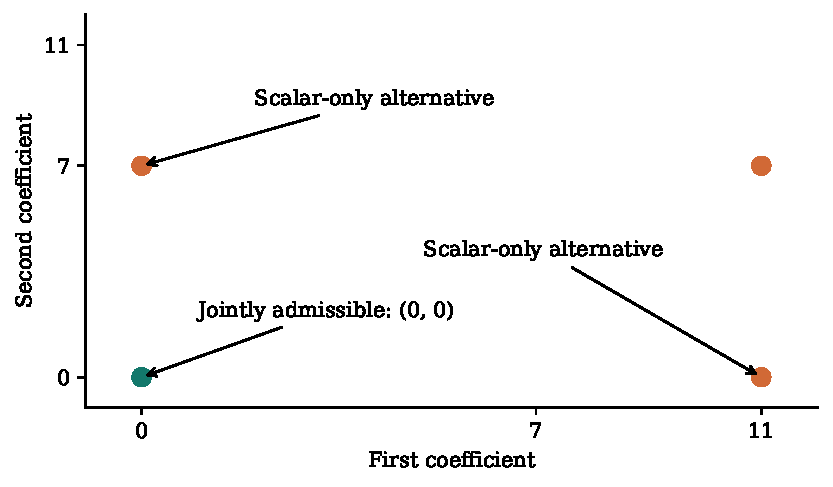
\includegraphics[width=.82\linewidth]{../figures/joint.pdf}
\caption{A prime-modulus example with $(m_1,m_2,m_3)=(5,7,11)$, $r_1=(1,2)$, $r_2=r_3=(0,0)$, and box $[0,11]^2$. The scalar candidate sets are $\{0,11\}$ and $\{0,7\}$, yielding four Cartesian combinations. Only $(0,0)$ has a single admissible fault explanation across both coordinates. The orange points do not have compatible common explanations.}
\label{fig:joint}
\end{figure}

\section{Number-field norm experiments}
\subsection{Objects and independent algebraic controls}
We use $K_d=\mathbb Q[t]/(f_d)$ with $f_d(t)=t^d-t-1$, for $d\in\{4,8,12,16\}$. These are number fields by Selmer's irreducibility theorem \cite{selmer}; the script also checks irreducibility. For each degree, twelve coefficient vectors are drawn uniformly from $\{-3,\ldots,3\}^d$ using the fixed seed 6312028. They specify $g(t)=\sum_{j=0}^{d-1}c_jt^j$ and the norm polynomial
\begin{equation}\label{eq:norm}
 N_g(X)=\operatorname{Norm}_{K_d/\mathbb Q}(X-g(\alpha))
       =\operatorname{Res}_t(f_d(t),X-g(t)).
\end{equation}
Let $A_g$ be multiplication by $g(\alpha)$ in the power basis. We independently compare the full symbolic resultant with $\det(XI-A_g)$ using SymPy 1.14.0. All 48 pairs agree exactly. Modular images are computed by a separate Faddeev--LeVerrier recurrence in $\mathbb F_p$, not by reducing a symbolic resultant. All 2,304 images agree with the exact coefficients modulo their primes. The leading monic coefficient is omitted from reconstruction.

The intervals are obtained before inspecting reconstruction outcomes. Let $R$ be the largest absolute row sum of $A_g$. Every eigenvalue has modulus at most $R$. For the coefficient of $X^{d-k}$, elementary symmetric functions therefore give
\begin{equation}\label{eq:bounds}
 |[X^{d-k}]N_g|\le B_k:=\binom dk R^k,\qquad k=1,\ldots,d.
\end{equation}
We declare $[-B_k,B_k]$; these bounds are conservative but analytic, and use neither the exact answer nor tuned empirical quantiles. If $R=0$ the intervals reduce to zero. The baseline and joint methods receive exactly the same intervals.

\subsection{Fault and placement grid}
Each object is evaluated at the first 48 primes starting at 101. All primes exceed the matrix dimensions, so the modular recurrence's divisions by $1,\ldots,d$ are invertible. These small primes make stopping differences visible; they do not model an optimized machine-word implementation.

Six source domains receive the images under two fixed layouts. Round robin assigns position $i$ to $i\bmod6$ using zero-based positions. Blocked placement assigns eight consecutive positions per source. For a budget $f\in\{1,2\}$, the faulty source IDs are $(s+h)\bmod6$, $h=0,\ldots,f-1$, where $s$ is the instance number. Unrepresented source domains at an early prefix contribute empty supports; duplicate unions are removed. Three controlled fault mechanisms are used:
\begin{enumerate}
\item \textbf{Dense random:} every coefficient in an affected image receives an independently drawn nonzero residue increment. Randomness is only an experimental mechanism, not a theorem assumption.
\item \textbf{Coherent wrong input:} affected sources return the coefficients associated with $g+1$, computed from $A_g+I$. The returned images are mutually consistent with a different algebraic input.
\item \textbf{Single coefficient:} only the constant coefficient is incremented by one at affected positions.
\end{enumerate}
The full grid is $4$ degrees $\times12$ objects $\times3$ mechanisms $\times2$ placements $\times2$ budgets, giving 576 configurations. The 48 underlying objects are reused across conditions; the configurations are not 576 independent random mathematical objects.

\subsection{Stopping rules and results}
At each prefix of the prime list we record the first success of three rules:
\begin{enumerate}
\item \textbf{Joint exact:} Theorem~\ref{thm:boxes} has a unique vector, and its certificate passes the separate verifier.
\item \textbf{Scalar exact:} every coordinate separately has a unique feasible value under the same support family and interval. This is a complete scalar information test, not a heuristic CRT decoder.
\item \textbf{Universal:} \eqref{eq:threshold} holds for the prefix's source-support family and maximum coefficient width.
\end{enumerate}
The code additionally records the sufficient product stopping point with the actual faulty domains disclosed (\texttt{clean} in the CSV). This is an oracle diagnostic, not a deployable competitor and not necessarily the earliest point of unique recovery with known faults.

All rules terminate within 48 primes. Every accepted vector equals the independently obtained exact norm polynomial. Joint stopping averages 15.519 prime computations, scalar stopping 16.116, and the universal rule 23.906. Summed across the grid, joint certification uses 3.71\% fewer primes than scalar certification and 35.08\% fewer than the universal bound. It improves on scalar stopping in 182/576 configurations and on the universal bound in 575/576. The maximum scalar saving is six primes. These are finite-benchmark counts; no population-level significance or wall-clock acceleration is inferred.

\begin{table}[tb]
\centering\small
\begin{tabular}{lrrrrr}\toprule
Mechanism & Cases & Joint & Scalar & Universal & Joint $<$ scalar\\\midrule
Dense random & 192 & 14.036 & 15.083 & 23.906 & 104 \\
Coherent wrong input & 192 & 15.911 & 16.656 & 23.906 & 78 \\
Single coefficient & 192 & 16.609 & 16.609 & 23.906 & 0 \\
\bottomrule\end{tabular}

\caption{Mean prime computations at stopping, stratified by fault mechanism. Each row reuses the same 48 mathematical objects across placements and budgets.}
\label{tab:modes}
\end{table}

\begin{table}[tb]
\centering\small
\begin{tabular}{lrrrrr}\toprule
Placement & $f$ & Cases & Joint & Scalar & Universal\\\midrule
Round robin & 1 & 144 & 8.910 & 9.583 & 11.708 \\
Round robin & 2 & 144 & 11.361 & 12.465 & 21.958 \\
Blocked & 1 & 144 & 15.479 & 15.688 & 23.021 \\
Blocked & 2 & 144 & 26.326 & 26.729 & 38.938 \\
\bottomrule\end{tabular}

\caption{Mean stopping counts by placement and allowed source failures. Blocking delays evidence from additional domains; these counts do not include parallel scheduling time.}
\label{tab:layouts}
\end{table}

\begin{figure}[tb]
\centering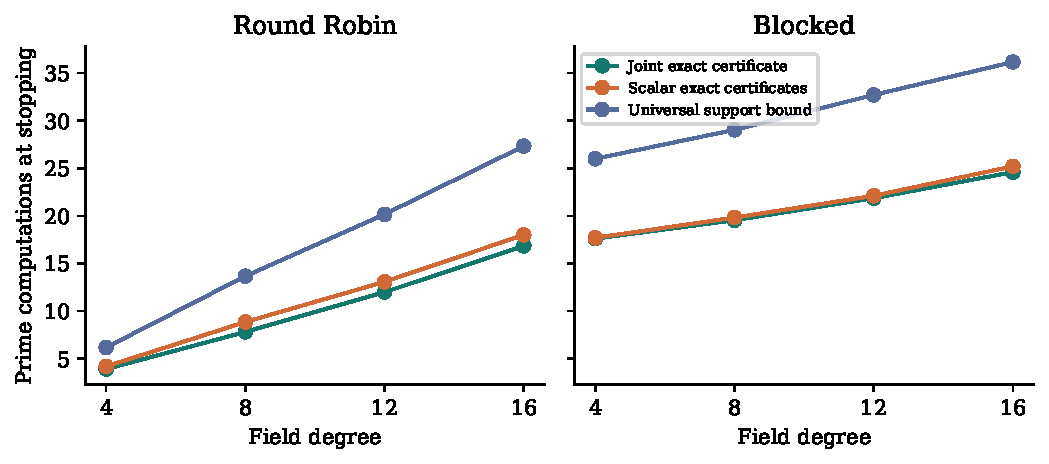
\includegraphics[width=\linewidth]{../figures/stopping.pdf}
\caption{Stopping counts by field degree and placement, averaged over the twelve objects, three mechanisms, and two fault budgets. Joint and scalar certification use the same information model; the universal rule protects every possible received array. Lines summarize this fixed grid rather than fitted scaling laws.}
\label{fig:stopping}
\end{figure}

\begin{figure}[tb]
\centering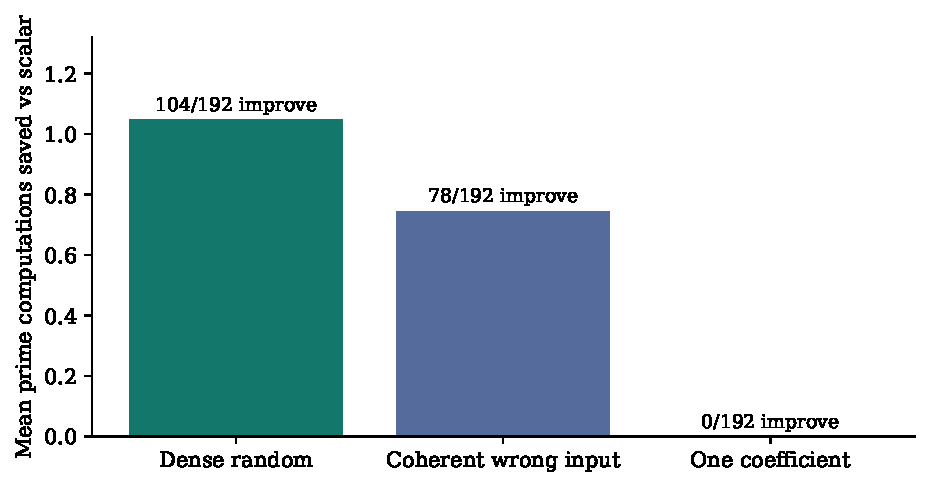
\includegraphics[width=.86\linewidth]{../figures/modes.pdf}
\caption{Savings against exact scalar certification. Dense and coherent vector errors sometimes allow different coefficients to eliminate different supports. Single-coefficient corruption gives no saving anywhere in this grid. Labels count improving configurations, not independent objects.}
\label{fig:modes}
\end{figure}

The zero saving for single-coefficient errors is a substantive negative control. Clean coordinates supply no additional contradiction against an alternative fault hypothesis: any such hypothesis still sees their correct values. The damaged coordinate determines stopping. Dense and coherent mechanisms can instead make different coordinates reject different hypotheses. Coherent wrong-input errors are more difficult than dense random errors on average, consistent with their algebraic structure.

Blocked placement averages 20.903 joint primes versus 10.135 under round robin. A prefix of a blocked sequence is concentrated in few fault domains. This demonstrates a property of the selected ordering and source model, not a universal recommendation to schedule by round robin or a comparison of equal wall-clock budgets. Proposition~\ref{thm:balance} gives a separate worst-case guarantee for information-aware least-load placement; the norm experiment does not claim that round robin optimizes it.

\section{Verification, reproducibility, and failure boundaries}
\subsection{Exact checks}
The small-case test suite enumerates all 4,500 received two-coordinate arrays for moduli $(2,3,5)$ and $(3,4,5)$ under one faulty singleton source. The boxes are $[-2,3]\times[-1,2]$. Direct enumeration of every point in each box agrees with all three classifications from the progression algorithm. The second modulus set also checks the allowance of composite, pairwise coprime moduli.

The suite checks 100 members of Proposition~\ref{thm:family}, validates the prime example in Figure~\ref{fig:joint}, and tests the universal threshold using overlapping source supports on moduli $(2,3,5,7)$. It includes empty clean sets, zero-width intervals, invalid noncoprime moduli, and an ambiguity construction at the threshold. These finite checks supplement the proofs, not replace them.

All 576 saved norm certificates are verified from their original declarations. Three deliberate mutations per certificate alter a candidate coefficient, delete a support record, or use an invalid exclusion coordinate. All 1,728 mutations are rejected. This is a specific mutation suite, not a claim that every malformed certificate has been enumerated. The verifier uses a different CRT construction from the producer and remains active under optimized Python execution.

The placement audit tests 1,200 cases spanning image counts $5,10,20,40$, source counts $3,5,8$, every positive budget satisfying $2f<h$, and fifty fixed-seed repetitions. The moduli are distinct-prime powers with exponents between one and eight. For each case, exact integers verify \eqref{eq:sourceproduct}, the least-load range bound, and the equivalent inequality
\begin{equation}
 S^h\,m_{\max}^{k(h-k)}\ge M^{h-k}.
\end{equation}
No floating-point logarithms are used in these checks.

\subsection{What a valid certificate cannot establish}
The verifier proves a conditional arithmetic statement. An explicit test makes this boundary visible: with moduli $(5,7,11)$, interval $[0,1]$, and a one-source budget, received values $(1,1,1)$ certify output one. If the physical truth were zero and all three workers failed coherently, that certificate would still be valid for the declared model and wrong about the physical computation. The premise, rather than the arithmetic certificate, would have failed.

The same issue applies to incorrect interval bounds, shared input corruption, wrong provenance labels, and an omitted common backend. Certificates do not authenticate who ran a computation. The declaration must be tied to a job manifest or other external provenance mechanism if used in a service. Independent replay can provide additional evidence, but its independence must also be justified externally.

The present output model is a Cartesian interval box of integers. Rational coefficients, unknown denominators, and algebraic relations among coefficients are outside the implementation. Encoding a rational vector by scaled integers is legitimate only with an independently justified common denominator. A large support family remains expensive; enumeration is designed for small numbers of domains and does not compete asymptotically with lattice decoders.

\subsection{Artifact and execution}
The public artifact contains the dependency-free reconstruction package, a separate verifier, tests, deterministic experiment scripts, full per-configuration CSV, all certificates, vector figures, and this \LaTeX{} source. The experiments use Python 3.12.14, SymPy 1.14.0, NumPy 2.5.4, and Matplotlib 3.11.2. Core correctness uses only Python integers and the standard library. A minimal reproduction is
\begin{lstlisting}
python -m pip install -e '.[experiments]'
python -m unittest discover -s tests -v
python experiments/run.py
python experiments/audit.py
python experiments/make_tables.py
cd paper && tectonic main.tex
\end{lstlisting}
Scripts assert exact agreement with controls and write the data underlying each figure. Timings in the CSV are diagnostic single-run measurements and are not compared in the paper. No measured cluster throughput, fault rate, or commercial revenue is claimed.

\section{Practical use and research directions}
A modular algebra service could expose the certificate together with its result and a small provenance manifest. A client could then distinguish a result that is unique under a declared source budget from one accepted only because coefficients stabilized. Number-field norm and characteristic-polynomial computations are natural initial workloads; they produce many integer coefficients sharing the same modular task provenance. The certificate format also separates an untrusted candidate proposer from a deterministic acceptance step.

This suggests a concrete engineering path: group images by actual backend and job lineage, derive justified coefficient bounds, generate a candidate using an existing fast method, and run exact source-family certification when the domain count is small. If the test is ambiguous, obtain additional images on another domain or strengthen the independently justified bounds. The sharp product threshold supplies a worst-case stopping diagnostic, while the instance certificate may stop earlier.

The commercial opportunity is a verifiable result interface for outsourced exact computation, rather than an assumed new market for a novel CRT decoder. Integration costs, provenance authentication, large-integer performance, and customer demand remain unmeasured. No patentability or market-size claim follows from these experiments. The broad CRT and interleaving precedents are particularly relevant to any future intellectual-property assessment.

Several research problems remain. One is to avoid full support enumeration while preserving complete instance certificates for overlapping domain hierarchies. Another is to combine source-information balancing with unequal prime costs and parallel latency. A third is to exploit polynomial coefficient relations without making the verifier as complex as the original algebraic computation. Finally, an integration with an established modular computer algebra backend should compare end-to-end performance and certificate overhead against existing guaranteed verification methods and interleaved decoding.

\section{Conclusion}
Bounded modular reconstruction depends on which collections of errors the computation is prepared to tolerate. A finite source-support family makes this assumption explicit. Cartesian CRT progressions then provide a complete instance audit and a certificate verifiable by exact arithmetic. The smallest clean product outside two explanations characterizes the universal uniqueness threshold, while joint coefficient exclusions can certify instances far beyond that bound. The norm-polynomial experiments establish this effect on a reproducible algebraic workload and identify a sparse-error regime with no benefit. The result is a small-source certification method with explicit assumptions, rather than an unconditional fault-tolerance guarantee.

\begin{thebibliography}{10}
\bibitem{stone} J. J. Stone. Multiple-burst error correction with the Chinese remainder theorem. \emph{Journal of the Society for Industrial and Applied Mathematics} 11(1), 74--81, 1963. \href{https://doi.org/10.1137/0111005}{doi:10.1137/0111005}.
\bibitem{grs} O. Goldreich, D. Ron, and M. Sudan. Chinese remaindering with errors. \emph{IEEE Transactions on Information Theory} 46(4), 1330--1338, 2000. Author version: \url{https://eprint.iacr.org/1999/002}.
\bibitem{boehm} J. B\"ohm, W. Decker, C. Fieker, and G. Pfister. The use of bad primes in rational reconstruction. \emph{Mathematics of Computation} 84(296), 3013--3027, 2015. \href{https://doi.org/10.1090/mcom/2951}{doi:10.1090/mcom/2951}. \url{https://arxiv.org/abs/1207.1651}.
\bibitem{abbott} J. Abbott. Fault-tolerant modular reconstruction of rational numbers. \emph{Journal of Symbolic Computation} 80, 707--718, 2017. \href{https://doi.org/10.1016/j.jsc.2016.07.030}{doi:10.1016/j.jsc.2016.07.030}.
\bibitem{lsn} W. Li, V. Sidorenko, and J. S. R. Nielsen. On decoding interleaved Chinese remainder codes. \emph{2013 IEEE International Symposium on Information Theory}, 1052--1056, 2013. \href{https://doi.org/10.1109/ISIT.2013.6620387}{doi:10.1109/ISIT.2013.6620387}.
\bibitem{basson} D. Basson, J. B\"ohm, M. S. Marais, M. Rahn, and H. P. Rakotoarisoa. Massively parallel modular methods in commutative algebra and algebraic geometry. 2024. \url{https://arxiv.org/abs/2401.11606}.
\bibitem{minpoly} J. Abbott, A. M. Bigatti, E. Palezzato, and L. Robbiano. Computing and using minimal polynomials. \emph{Journal of Symbolic Computation}, 2019. Revised author version: \url{https://arxiv.org/abs/1702.07262}.
\bibitem{graham} R. L. Graham. Bounds for certain multiprocessing anomalies. \emph{Bell System Technical Journal} 45(9), 1563--1581, 1966. \href{https://doi.org/10.1002/j.1538-7305.1966.tb01709.x}{doi:10.1002/j.1538-7305.1966.tb01709.x}.
\bibitem{selmer} E. S. Selmer. On the irreducibility of certain trinomials. \emph{Mathematica Scandinavica} 4, 287--302, 1956. \href{https://doi.org/10.7146/math.scand.a-10478}{doi:10.7146/math.scand.a-10478}.
\end{thebibliography}
\end{document}
